\batchmode
\documentclass{beamer}
\usepackage[utf8]{inputenc}
\usepackage[ngerman]{babel}

\usetheme[deutsch]{KIT}
\author{Jan Haag (jan.haag@student.kit.edu)}
\title{Programmieren Tutorium 1 -- Klassen und Objekte}
\institute{Institut f\"{u}r Zeritfizierbare und Vertrauensw\"{u}rdige Informatiksysteme (ZVI)}
\TitleImage[scale=0.225]{frontpic.jpg}

\begin{document}
\begin{frame}
\maketitle
\end{frame}

\begin{frame}
\frametitle{Inhalt}
\tableofcontents
\end{frame}

\section{Organisatorisches}
\begin{frame}[fragile]
\frametitle{Wichtige Daten}
\begin{description}
\item[Folienarchiv] \verb|https://github.com/janhaag/progtut2011|
\item[Fragen]
\begin{itemize}
\item Praktomat-Forum
\item Mir eine Mail schreiben (jan.haag@student.kit.edu)
\end{itemize}
\end{description}
\end{frame}

\section{Java -- Installation und Verwendung}
\begin{frame}[fragile]
\frametitle{Java -- Installation}
\begin{description}
\item[JDK Installation]
\begin{description}
\item[Windows] Download des Installers von der Java Download-Seite
\item[Linux] Die meisten Distributionen haben das OpenJDK oder das Oracle JDK in ihren Repositories
\item[Mac OS X] Das JDK wird zusammen mit den XCode Developer Tools von der Installations-DVD installiert.
\end{description}
\end{description}
\end{frame}

\begin{frame}[fragile]
\frametitle{Java -- Installation}
\begin{description}
\item[Editoren]
\begin{description}
\item[Windows] Notepad++, Vim
\item[Linux] Vim, Emacs, Kate, gEdit, ...
\item[Mac OS X] MacVim, XCode, TextMate, ...
\end{description}
\item[Java Docs] Download von der Java Download-Seite
\item[Java Downloads] \verb|http://www.oracle.com/technetwork/java/|$\hookleftarrow$\\
\verb|javase/downloads/index.html|
\end{description}
\end{frame}

\begin{frame}
\frametitle{Funktion des JDK}
\end{frame}

\section{Java -- Funktion}
\begin{frame}[fragile]
\frametitle{Aufbau einer Klasse}
\begin{verbatim}
public class Example {
    Typ attribut1;
    int zahl = 1;
}
\end{verbatim}
\end{frame}

\subsection{Aufgaben}
\begin{frame}
\frametitle{Modellierung eines Autos}
Was macht ein Auto aus? Modelliere es durch passende Klassen und Objekte.
\end{frame}

\begin{frame}[fragile]
\frametitle{Theorie...}
Werten Sie folgende Ausdr\"{u}cke aus.
\begin{verbatim}
boolean a = true;
boolean b = false;
boolean c = true;
boolean d;
d = !a;
d = a && b;
d = !a || !c;
d = (a && b) || !c;
\end{verbatim}
\end{frame}

\begin{frame}[fragile]
\frametitle{Theorie...}
Werten Sie folgende Ausdr\"{u}cke aus.
\begin{verbatim}
int i = 2;
double d = 3.14;
// Betrachten Sie die Zeilen unabhaengig voneinander
int result = i + 12;
double result = i / 5;
int result = i / 6;
int result = 7 % i;
int result = 7 / i;
double result = i / d;
double result = 2 / 3;
double result = 2 / 3.0;
\end{verbatim}
\end{frame}

\begin{frame}
\frametitle{Ende}
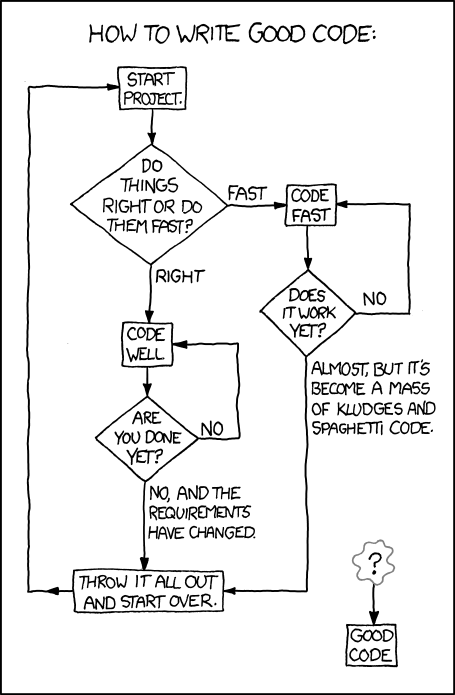
\includegraphics[scale=0.25]{good_code.png}
\end{frame}
\end{document}
